% ========================================= TEMPLATE INFO ========================================
%
% Author:       P4ntomime
% Version:      1.0.1
% Last updated: 2026-01-24
% Brief:        A LaTeX template for summaries. See README.md for more information.
% 
% ================================================================================================
\documentclass[8pt, a4paper, twoside]{extarticle}
% Font size:    8pt
% Paper size:   A4
% style:        twoside (needed, so odd and even pages have different margins)
% orientation:  portrait. (use 'landscape' for landscape orientation)


% ========================================= DOCUMENT INFO =========================================
\def\title{ComEng - Ergänzung}      % Titel
\def\shorttitle{ComEng}             % Kurztitel (angezeigt als PDF-Titel)
\def\dozent{Prof. Lars Kamm}        % Dozent
\def\semester{FS 2026}              % Semester
\def\author{Mirko Ratti}            % Autor(en)
% \def\contributors{Contributors}   % contributor(s) (optional -> comment out if none)
\def\repo{https://github.com/mirkoratti/FS2026} % Repository-Link
\def\version{1.0.\today}            % Version
\def\pagelimit{3}                   % Seitenlimit -> führt dazu, dass Seiten nach dem Limit rot werden
\def\titleoption{normal}            % Optionen: ultra kompakt, kompakt, normal
\def\enableToC{true}                % Aktivieren/Deaktivieren des Inhaltsverzeichnisses

% ================================= PACKAGES, SETUP AND COMMANDS ==================================
\input{preamble.tex}


% =========================================== DOCUMENT ============================================
\begin{document}
    \begin{layout}
        \section[Hex - Dez]{Hex $\to$ Dez}
\begin{ctabular}{l|cccccc}
    \textbf{Hex} & A & B & C & D & E & F \\
    \textbf{Dec} & 10 & 11 & 12 & 13 & 14 & 15 \\
    \textbf{Bin} & 1010 & 1011 & 1100 & 1101 & 1110 & 1111
\end{ctabular}\vspace{-1em}

\section{Instruction Set Architecture (ISA)}
\label{subsec:isa_differences}

Die Weiterentwicklung der ARM-Architekturen hat zur Koexistenz verschiedener Befehlssätze geführt.

\begin{itemize}
    \item \textbf{ARM (32-bit) (Veraltet):} 32 Bit, maximale Leistung, aber sie belegen mehr Speicherplatz.
    \item \textbf{Thumb (16-bit):} Untermenge 16 Bit,
    Ideal, um den Speicher-Footprint zu reduzieren (ca. 30\% Einsparung)
    \item \textbf{Thumb-2 (16/32-bit):} variable Länge (16 und 32 Bit). Ermöglicht eine Code-Dichte ähnlich zu Thumb 
    mit vergleichbarer Leistung wie der 32-Bit-ARM-Befehlssatz.
\end{itemize}

\section{Logik der ALU und Program Status Register}
\label{sec:alu_logic}

Die Arithmetisch-Logische Einheit (ALU) arbeitet ausschließlich auf binären Bitfolgen, 
ohne die Semantik des Vorzeichens zu berücksichtigen (Interpretation \textit{signed} vs \textit{unsigned}).

\subsection{Flag-Mechanismus (APSR)}
\label{subsec:apsr_flags}

\begin{itemize}
    \item \textbf{N (Negative):} Spiegelt das höchstwertige Bit (MSB) des Ergebnisses wider. Wenn $MSB=1$, wird das Flag auf 1 gesetzt.
    \item \textbf{Z (Zero):} Auf 1 gesetzt, wenn alle Bits des Ergebnisses gleich 0 sind.
    \item \textbf{C (Carry):} Zeigt einen Übertrag über das höchstwertige Bit hinaus an. 
\begin{itemize}
    \item Entscheidend für Operationen \textit{unsigned}. \crd{Für die Subtraktion invertiert!}
    \item \textbf{Subtraktions-Mechanismus:} $(A + \text{NOT}(B) + 1)$. \quad Zweierkomplement.
\begin{itemize}
        \item $C = 1 \implies A \ge B$ (Kein Borrow / Not-Borrow).
        \item $C = 0 \implies A < B$ (Borrow erfolgt / Borrow).
    \end{itemize}
\end{itemize}
    \item \textbf{V (oVerflow):} Zeigt einen Vorzeichenfehler in der Rechnung im Zweierkomplement an 
    und ist entscheidend für Operationen \textit{signed}.
\begin{itemize}
        \item $(+) + (+) = (-)$ Unmöglich
        \item $(-) + (-) = (+)$ Unmöglich
    \end{itemize}
\end{itemize}

\subsubsection{Interpretation des Vorzeichens und bedingte Sprünge}
\label{subsec:sign_interpretation}

Da die ALU gleichzeitig sowohl das Flag $C$ als auch das Flag $V$ aktualisiert,
liegt die Unterscheidung zwischen der Variable \texttt{int} und \texttt{uint} nicht in der Hardware, 
sondern in der Software.


        \input{sections/02_sistema_controllo.tex}
        % --- SEZIONE 2: MODELLO DI MEMORIA E STACK ---
\section{Ottimizzazione e Strutture Dati}

\subsubsection{Switch Case}
\begin{itemize}
    \item \textbf{Pro:} Anzahl der Taktzyklen definiert und vorhersehbar.
    \item \textbf{Contra:} Die Bedingung muss notwendigerweise eine Konstante vom Typ \texttt{int} sein.
    \item \textbf{Hinweis:} Die Reihenfolge der \texttt{case} ist für die Effizienz der Suche relevant.
\end{itemize}

\subsubsection{Flusso di Controllo in Assembly}
\begin{itemize}
    \item \textbf{Selektionen (If/Else):} Es wird ein \textbf{Sprung nach vorn} mit der \textbf{invertierten Bedingung} gegenüber C verwendet (wenn die Bedingung falsch ist, springt man über den \textit{then}-Block hinaus).
    \item \textbf{Iterationen (Loop):} Es wird ein \textbf{Sprung nach hinten} am Ende der Schleife verwendet, wobei die \textbf{Assembly-Bedingung wie in C} beibehalten wird (Sprung zum Anfang, wenn die Bedingung noch wahr ist).
\end{itemize}

% \subsubsection{Tecniche di Ottimizzazione}
% \begin{itemize}
%     \item \textbf{Loop Unrolling:} Tecnica che consiste nel ripetere il corpo del loop 
%     per ridurre l'overhead dei \textit{branch} e degli incrementi del contatore.
%     \texttt{\#pragma unroll (n)}
%     \item \textbf{Pointers (Stackless):} L'uso dei registri invece dello stack per manipolare i puntatori è significativamente più veloce (spesso più del doppio).
% \end{itemize}

\subsubsection{Efficienza delle Strutture Dati}
\begin{itemize}
    \item \textbf{Lokale Arrays:} Sehr \textbf{ineffizient}. 
    hohe Anzahl von Zyklen nur für die Initialisierung im Stack-Frame 
    \item \textbf{Strukturen:} Es ist empfehlenswert, die \textbf{Strukturen global zu definieren}. Die lokale Initialisierung auf dem Stack führt zu einem hohen Overhead an Taktzyklen.
    \item \textbf{Bitfields:} Extrem \textbf{ineffizient}. 
    Obwohl sie Speicher sparen, erfordern sie komplexe Operationen von
     \textit{Read-Modify-Write} (LDR, Shift, Mask, OR, STR)
\end{itemize}
        % --- SEZIONE 3: ARCHITETTURE E COMPILAZIONE ---

\section{Confronto Architetture ARM Cortex}
\begin{description}
    \item[Cortex-A (Application):] Generische Berechnung mit hoher Leistung (Linux/Android).
    \item[Cortex-R (Real-Time):] Geringe Latenz und hohe Zuverlässigkeit (Automotive/Medizin).
    \item[Cortex-M (Microcontroller):] Reduzierter Energieverbrauch, deterministische Interrupts.
\end{description}

\renewcommand{\arraystretch}{1.5}
\resizebox{\columnwidth}{!}{
\begin{tabular}{|l|c|c|c|c|c|c|c|c|}
\hline
\textbf{Core} & \textbf{Thumb} & \textbf{Thumb-2} & \textbf{HW Mult.} & \textbf{HW Div.} & \textbf{Math Sat.} & \textbf{DSP} & \textbf{FPU} & \textbf{Arch} \\
\hline
Cortex-M0  & \cellcolor{green!60}Mostly & \cellcolor{green!60}Subset & \cellcolor{green!60}1/32 cyc & \cellcolor{red!60}No & \cellcolor{red!60}No & \cellcolor{red!60}No & \cellcolor{red!60}No & ARMv6-M \\
Cortex-M0+ & \cellcolor{green!60}Mostly & \cellcolor{green!60}Subset & \cellcolor{green!60}1/32 cyc & \cellcolor{red!60}No & \cellcolor{red!60}No & \cellcolor{red!60}No & \cellcolor{red!60}No & ARMv6-M \\
Cortex-M1  & \cellcolor{green!60}Mostly & \cellcolor{green!60}Subset & \cellcolor{green!60}3/33 cyc & \cellcolor{red!60}No & \cellcolor{red!60}No & \cellcolor{red!60}No & \cellcolor{red!60}No & ARMv6-M \\
Cortex-M3  & \cellcolor{green!60}Fully  & \cellcolor{green!60}Fully  & \cellcolor{green!60}1 cyc    & \cellcolor{green!60}Yes & \cellcolor{green!60}Yes & \cellcolor{red!60}No  & \cellcolor{red!60}No & ARMv7-M \\
Cortex-M4  & \cellcolor{green!60}Fully  & \cellcolor{green!60}Fully  & \cellcolor{green!60}1 cyc    & \cellcolor{green!60}Yes & \cellcolor{green!60}Yes & \cellcolor{green!60}Yes & \cellcolor{yellow!60}Optional & ARMv7E-M \\
Cortex-M7  & \cellcolor{green!60}Fully  & \cellcolor{green!60}Fully  & \cellcolor{green!60}1 cyc    & \cellcolor{green!60}Yes & \cellcolor{green!60}Yes & \cellcolor{green!60}Yes & \cellcolor{yellow!60}Optional & ARMv7E-M \\
\hline
\end{tabular}}
\renewcommand{\arraystretch}{1}

\subsection{Evoluzione Cortex-M0 vs M0+}
\begin{minipage}[t]{0.49\columnwidth}
    \begin{itemize}
        \item \textbf{M0+ Pipeline:} Auf 2 Stufen reduziert für höhere Effizienz.
        \item \textbf{I/O-Zugriff:} Unterstützung für Single-Cycle GPIO.
        \item \textbf{Debugging:} Optionaler Micro Trace Buffer (MTB) zum Nachverfolgen von Sprüngen.
        \item \textbf{MPU}
    \end{itemize}
\end{minipage}\hfill
\begin{minipage}[t]{0.49\columnwidth}
    \textbf{Pipeline}
    \begin{itemize}
        \item[+] Es wird in jedem Cycle ein Befehl ausgeführt
        \item [-] Bei Sprüngen muss die Pipeline 'geleert' werden
    \end{itemize}
\end{minipage}


\section{Adressierungsarten ARM (Cortex-M0)}
\begin{minipage}{0.5\columnwidth}
    \begin{itemize}
        \item Register direkt
        \item Register Indirekt
    \end{itemize}
\end{minipage}
\begin{minipage}{0.5\columnwidth}
    \begin{itemize}
        \item Register Indirekt mit offset \texttt{[R?, \#imm]}
        \item Register Indirekt mit index \texttt{[R?, R?]}
    \end{itemize}
\end{minipage}

\begin{minipage}[t]{0.5\columnwidth}
    \subsection{Register Direkt, Immediate}
    \begin{itemize}
        \item \textbf{Immediate:} \texttt{MOV R0, \#100} $\rightarrow$ Der Wert wird direkt geladen.
        \item \textbf{Register:} \texttt{MOVS R2, R1} $\rightarrow$ Kopiert den Wert zwischen Registern.
        \item \textbf{Einschränkungen:} Die Immediate-Werte werden in der Instruktion kodiert (z.B. 8-bit für \texttt{MOVS}).
    \end{itemize}

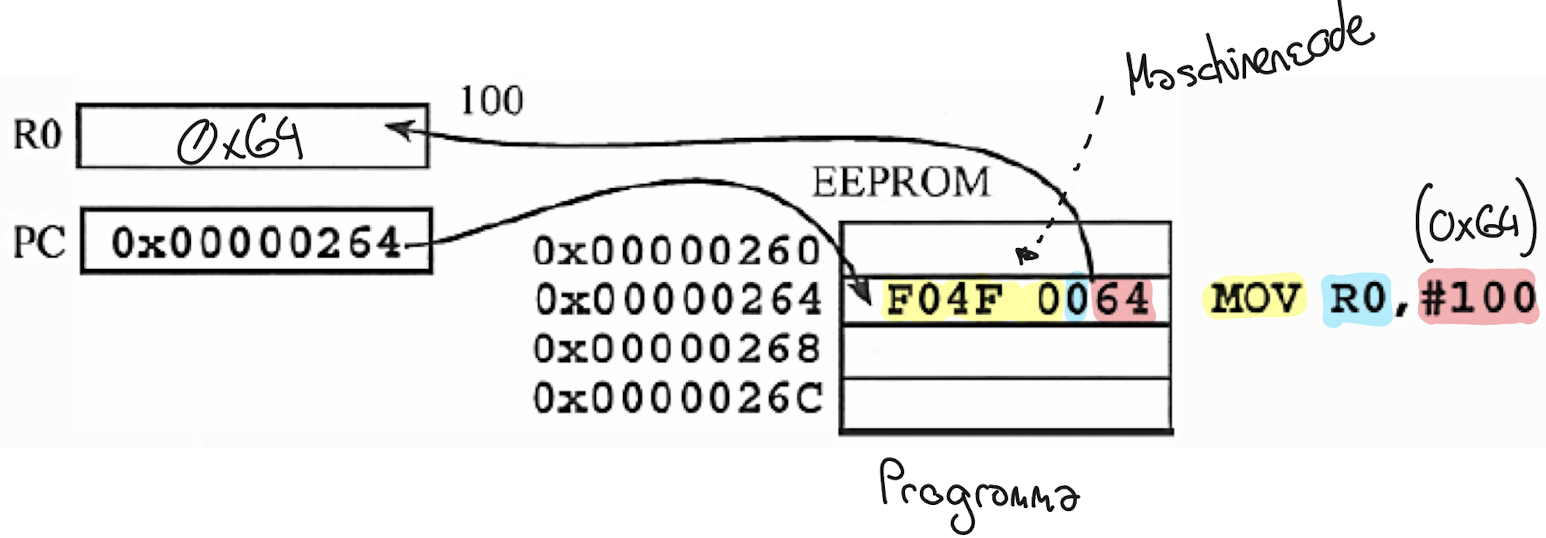
\includegraphics[width=\linewidth]{images/register_direkt.png}
\end{minipage}
\begin{minipage}[t]{0.5\columnwidth}
    \subsection{Register Indirekt (ptr)}
    \begin{itemize}
        \item \textbf{Einfach:} \texttt{LDR R0, [R1]} \\
        $\rightarrow$ $R0 = \text{Wert an der Adresse } R1$.
        \item \textbf{Mit Offset:} \texttt{LDR R0, [R1, \#4]} $\rightarrow$ $R0 = \text{Wert an der Adresse } R1 + 4$ (nützlich für Arrays/Structs).
        \item \textbf{Mit Index:} \texttt{LDR R0, [R1, R2]} \\
        $\rightarrow$ $R0 = \text{Wert an der Adresse } R1 + R2$.
    \end{itemize}    
    \begin{center}
        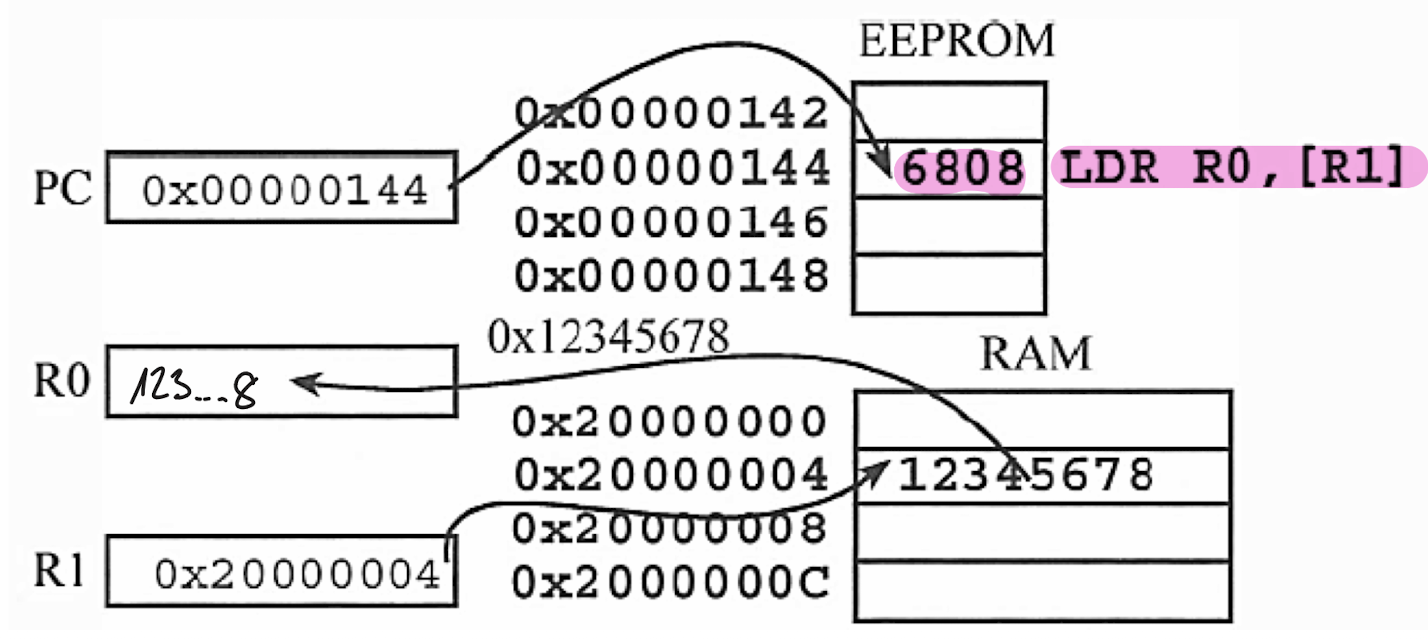
\includegraphics[width=\linewidth]{images/register_indirekt.png}
    \end{center}
\end{minipage}

\subsection{PC-Relative \& Literal Pool}
\begin{itemize}
    \item \textbf{Problem:} 32-bit-Instruktionen können keine 32-bit-Konstanten enthalten.
    \item \textbf{Lösung:} Der Assembler speichert die Konstante im \textbf{Literal Pool} (Speicherbereich in der Nähe).
    \item \textbf{Zugriff:} \texttt{LDR R0, =0x12345678} wird übersetzt in \texttt{LDR R0, [PC, \#offset]}.
    \item Es sind immer \textbf{zwei Speicherzugriffe} erforderlich
\end{itemize}

\subsection{Registerlisten \& Stack (SP-Relative)}
\begin{itemize}
    \item \textbf{Multiple:} \texttt{LDM R7!, \{R0-R3, R5\}} $\rightarrow$ Lädt mehrere Register beginnend bei der Adresse in $R7$.
    \item \textbf{Stack:} \texttt{PUSH \{R0-R2\}}, \texttt{POP \{R0-R2\}}.
    \item \textbf{Goldene Regel:} Das Register mit der niedrigsten Nummer (\texttt{R0}) geht immer in die niedrigste Speicheradresse. Die Reihenfolge in den geschweiften Klammern ist für die Hardware nicht relevant.
\end{itemize}

\subsection{Stack Framing}
Der Stack Frame ist der in RAM reservierte Bereich für lokale Variablen einer Funktion.

\begin{minipage}{0.5\columnwidth}
    \begin{itemize}
        \item \textbf{Allokation:} \texttt{SUB SP, SP, \#X} reserviert $X$ Byte (der Stack wächst zu niedrigeren Adressen).
        \item \textbf{Frame Pointer ($R7$):} Man verwendet \texttt{MOV R7, SP}, um einen festen Bezug zum Anfang des Frames zu haben.
        \item \textbf{Zugriff:} Die Variablen werden unter Verwendung von Offsets relativ zu $R7$ geschrieben/gelesen, z.B.: \texttt{STR R0, [R7, \#4]}.
        \item \textbf{Deallokation:} Vor dem Rücksprung (\texttt{BX LR}) muss der Stack mit \texttt{ADD SP, SP, \#X} bereinigt werden.
    \end{itemize}
\end{minipage}
\begin{minipage}{0.5\columnwidth}
    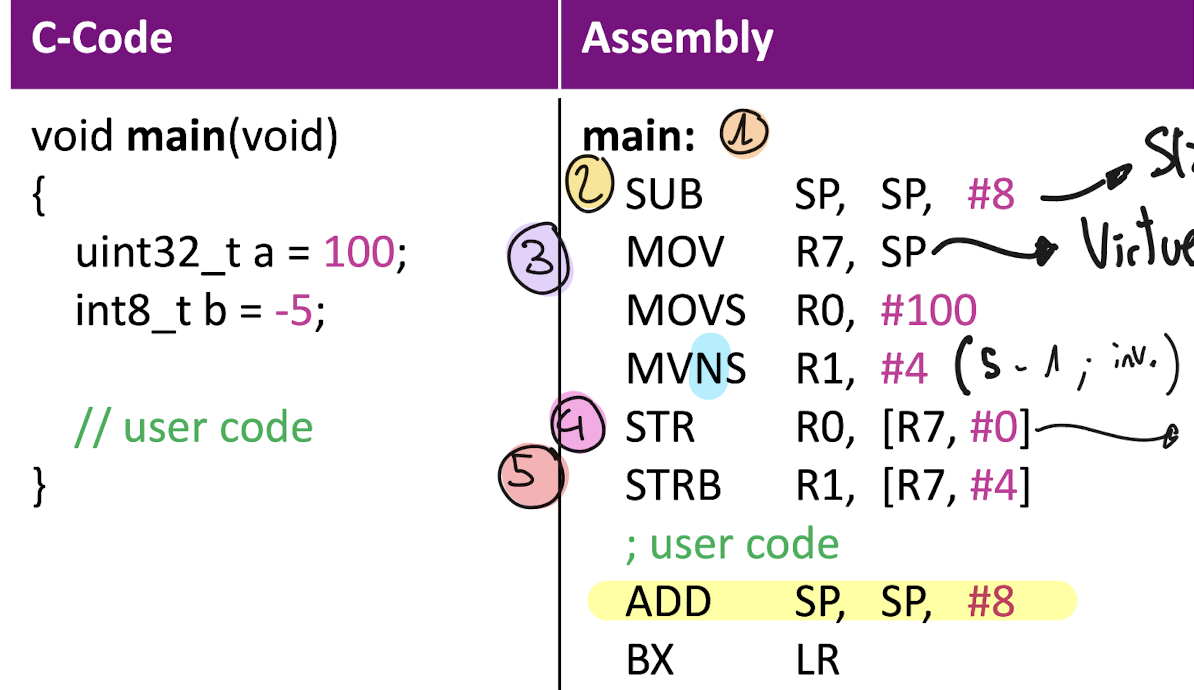
\includegraphics[width=\linewidth]{images/stack_framing.png}
\end{minipage}


        \section{Il Processo di Compilazione}
Der Quellcode wird durch verschiedene Phasen in Binärdaten umgewandelt:

\begin{enumerate}
    \item \textbf{Präprozessor:} Verarbeitet Einbindungen und Makros. (\texttt{\#define}, \texttt{\#if}, \dots)
    \item \textbf{Compiler:} Übersetzt die Sprache auf hoher Ebene in Assembly.
    \item \textbf{Assembler:} Konvertiert Assembly in relokierbaren Maschinencode.
    \item \textbf{Linker/Binder:} Verbindet Objektdateien und Bibliotheken.
    \item \textbf{Loader:} Konvertiert relokierbare Adressen in absolute und lädt sie in den Speicher.
\end{enumerate}

\subsection{Analisi del Compilatore}
\begin{itemize}
    \item \textbf{Lexikalische Analyse:} Entfernen von Leerzeichen und Gruppierung von Tokens.
    \item \textbf{Syntaktische/Semantische Analyse:} Prüfung der Struktur und der Datentypen.
    \item \textbf{Optimierung:} Verbesserung des Codes hinsichtlich Geschwindigkeit oder Speicherplatz.
    \item \textbf{Generierung:} Erzeugung des Zielcodes.
\end{itemize}

\section{Interfacciamento I/O}
Die Peripheriegeräte werden über spezifische Register in den Speicher abgebildet (\textit{Memory Mapped I/O}):
\begin{itemize}
    \item \textbf{Datenregister:} Enthält die zu verarbeitenden Daten.
    \item \textbf{Steuerregister:} Konfiguration des Peripheriegeräts.
    \item \textbf{Statusregister:} Zeigt den aktuellen Zustand des I/O (z. B. Busy, Ready) an.
\end{itemize}



        \input{sections/06_esempi.tex}
    \end{layout}
\end{document}